Jorge Pichardo ... \\[12pt]
Grupo C212\\
	Ciencia de la Computaci\'on\\
	Facultad de Matem\'atica y Computaci\'on\\
	Universidad de La Habana. Cuba\\
\and
Eisler F. Valles Rodriguez\\[12pt]
Grupo C211\\
    Ciencia de la Computaci\'on\\
	Facultad de Matem\'atica y Computaci\'on\\
	Universidad de La Habana. Cuba\\
\and
Autor IV\\[12pt]
Grupo C211\\
	Ciencia de la Computaci\'on\\
	Facultad de Matem\'atica y Computaci\'on\\
	Universidad de La Habana. Cuba\\
}



\maketitle
\section*{Tareas a realizar}
En el Informe debe Presentar:
\begin{itemize}
 \item Informe de la Tarea Investigativa II. T\'itulo del art\'iculo analizado
 \item Autores del trabajo.
 \item Resumen del trabajo.
 \item Intoducci\'on del trabajo debe de mensional, los autores del art\'iculo analizado, la revista donde se public\'o. A\~no. Factor de impacto de la revista. Valoraci\'on del art\'iculo: Explicaci\'on sobre lo que trata el art\'iculo, problem\'atica que se propone resolver, t\'ecnicas utilizadas.
 \item Otro ep\'igrafe para presentar las ecuaciones que ilustran el modelo matem\'atico utilizado. Condiciones iniciales o de frontera. Resultados a los que arriban. Ejemplos num\'ericos: Reproducci\'on de los algunos de los ejemplos o experimentos num\'ericos que se expliquen en el art\'iculo, utilizando para ello (RK4/Euler expl\'icito o impl\'icito) estudiado en clases y comparar resultados. Buscar puntos de equilibrio en caso de existir y analizar la estabilidad de dichos puntos. Pueden usarse para ello recursos computacionales. Presentar el diagrama de fases entre un par variables inc\'ognitas, valorando su comportamiento.
 \item Conclusiones: Una valoraci\'on de lo que usted ha aprendido con este trabajo, como valora la posibilidad de que se pueda continuar esta l\'inea de investigaci\'on.
 \item Bibliograf\'ia Consultada.
 \item  Anexos: Incluir seudo c\'odigos de sus programas.
 \item Valoraremos las iniciativas que presenten, como pueden ser, interfaces gr\'aficas, bases de datos, elementos  vinculen con otras asignaturas de la especialidad.
\end{itemize}

\section*{Estructura de la platilla}
\section*{Resumen}
Aqu\'i va el resumen del trabajo en esta plantilla  \LaTeX\ 

\section{INTRODUCCI\'ON}
\label{sec:intro}
Aqu\'i va la introducc\'on del trabajo en esta plantilla  \LaTeX\ 
\subsection{Estructura del trabajo}

\section{Resultados fundamentales.}

Muestre s\'olo las ecuaciones m\'as importantes y numere \'unicamente las ecuaciones mostradas a las que se hace referencia expl\'icita en el texto. \\

$\bar Y = n^{-1} \sum_{i=1}^n Y_i$\\
$$s^2 = \frac 1 {n-1} \sum_{i=1}^n (Y_i - \bar Y)^2.$$

\[
 c^2=a^2+b^2
\]

\begin{equation}\label{eq:quadratic}
ax^2 + bx + c = 0, \mbox{ donde } a \ne 0.
\end{equation}

En el texto, cada referencia a un n\'umero de ecuaci\'on debe ir tambi\'en entre par\'entesis. Por ejemplo, la soluci\'on de (\ref{eq:quadratic}) est\'a dada por  (\ref{eq:quadraticsol}) en los Axenos \ref{app:quadratic}.


\begin{equation} \label{eq:quadratic_second}
ax^2 + bx + c = 0
\end{equation}

\subsubsection{M\'etodos y algoritmos utilizados}
Esta  subsecci\'on se describen los c\'odigos de programas utilizados en el trabajo mediante las siguiente instrucciones.

\begin{verbatim}
y_{n+1}=y_n+hf(x_n,y_n}
\end{verbatim}


\begin{itemize}
	\item Utilice vi\~netas est\'andar en lugar de tildes, flechas, etc.
\end{itemize}
\begin{enumerate}
	\item En las listas numeradas, las etiquetas no deben ser n\'umeros ar\'abigos encerrados entre par\'entesis, \cite{simulation}
\end{enumerate}


\begin{table}[htb]
\centering
\caption{Uso de tabla\label{tab: first}}
\begin{tabular}{rll}
\hline
-& IQ & Dieta\\ \hline
- & 70 & Cualquier cosa\\
- & 60 &- \\
\hline
\end{tabular}
\end{table}

%\begin{figure}[htb]
%{
%\centering
%%\includegraphics[width=0.9\columnwidth]{MathExpandExpression.jpg}
%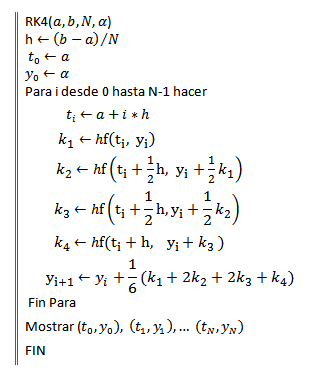
\includegraphics[width=0.50\textwidth]{alg_rk4}
%\caption{Figura-I.\label{fig: tahi}}
%}
%\end{figure}

.
\begin{definition}

\end{definition}

\begin{theorem}

\end{theorem}

\begin{corollary}

\end{corollary}

.



{\footnotesize
\begin{hangref}
\item Banks, J., J. S. Carson, B. L. Nelson, and D. M. Nicol. 2000. \textit{Discrete-Event System Simulation}. 3rd ed. Upper Saddle River, New Jersey: Prentice-Hall, Inc.
\end{hangref}
}




\bibliographystyle{wsc}
\bibliography{demobib}




\section*{Agradciemientos}


\appendix

\section{Anexos} \label{app:quadratic}

\begin{equation} \label{eq:quadraticsol}
x = \frac{-b \pm \sqrt{b^2-4ac}}{2a} \mbox{ si } a \ne 0.
\end{equation}


\end{document}

